\begingroup
\raggedright

\section{Nominal MPC}
\subsection{Constrained Finite Time Optimal Control (CFTOC)}
Solving \ref{eq:opt_standard_form} for an infinite horizon is \textbf{untractable}, that's why we solve it for a finite horizon N. $J^\star(x(k)) = \min_u I_f(x_N) + \sum^{N-1}_{i=0}I(x_i, u_i)$, where $I_f = x_N^{T}Px_N$ approximates the tail of the cost and $I = x_i^TQx_i + u_i^TRu_i$. This can be turned into a QP Problem of the form:

\begin{equation}
\begin{aligned}
\min_{z \in \mathbb{R}^n} \quad & \frac{1}{2}z^THz + q^Tz + r \\
\text{subj. to} \quad & Gz \leq h \\
& Az = b 
\end{aligned}
\end{equation}
\subsubsection{Without Substitution}
\begin{center}
\setlength{\tabcolsep}{1pt}
\renewcommand{\arraystretch}{0}
\begin{tabular}{cc}
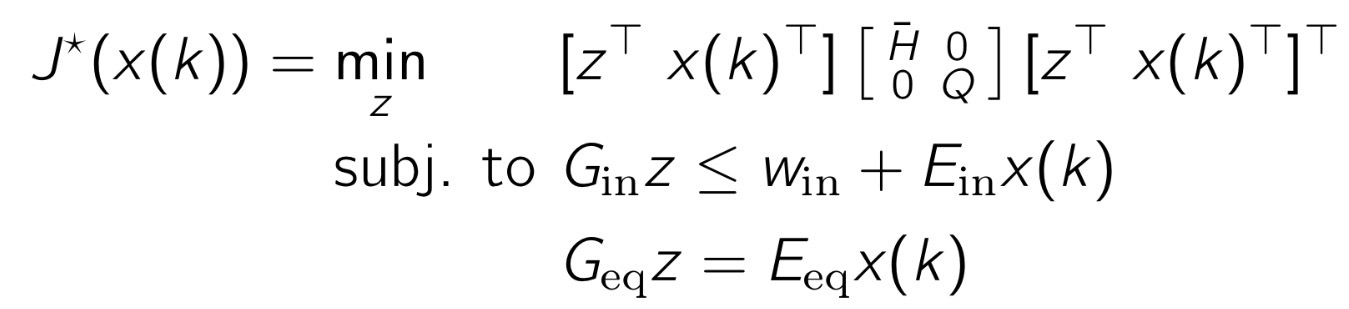
\includegraphics[width=0.49\linewidth]{images/CFTOC/without/problem.jpg} &
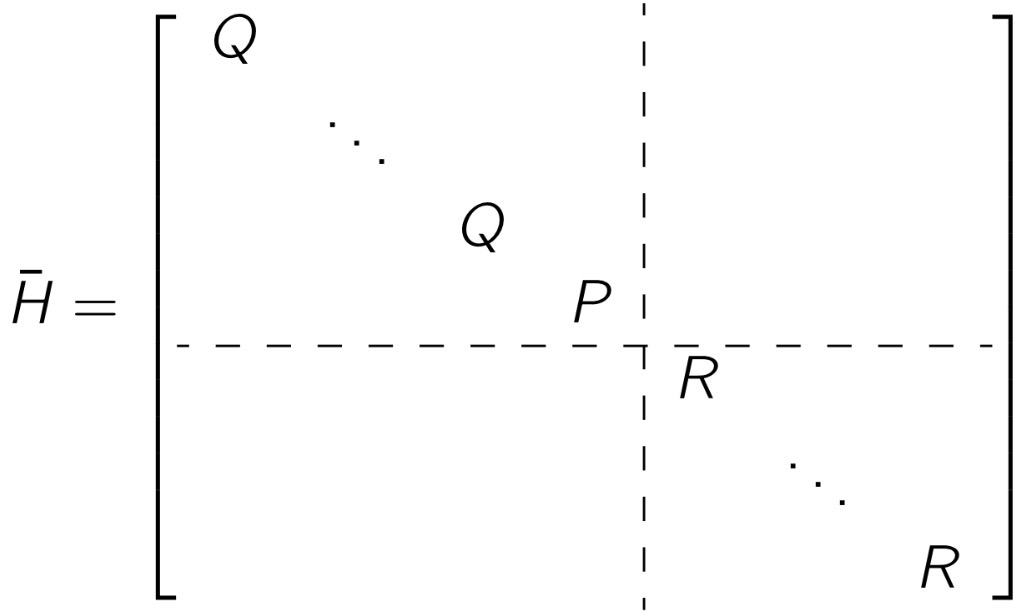
\includegraphics[width=0.29\linewidth]{images/CFTOC/without/H.jpg} \\
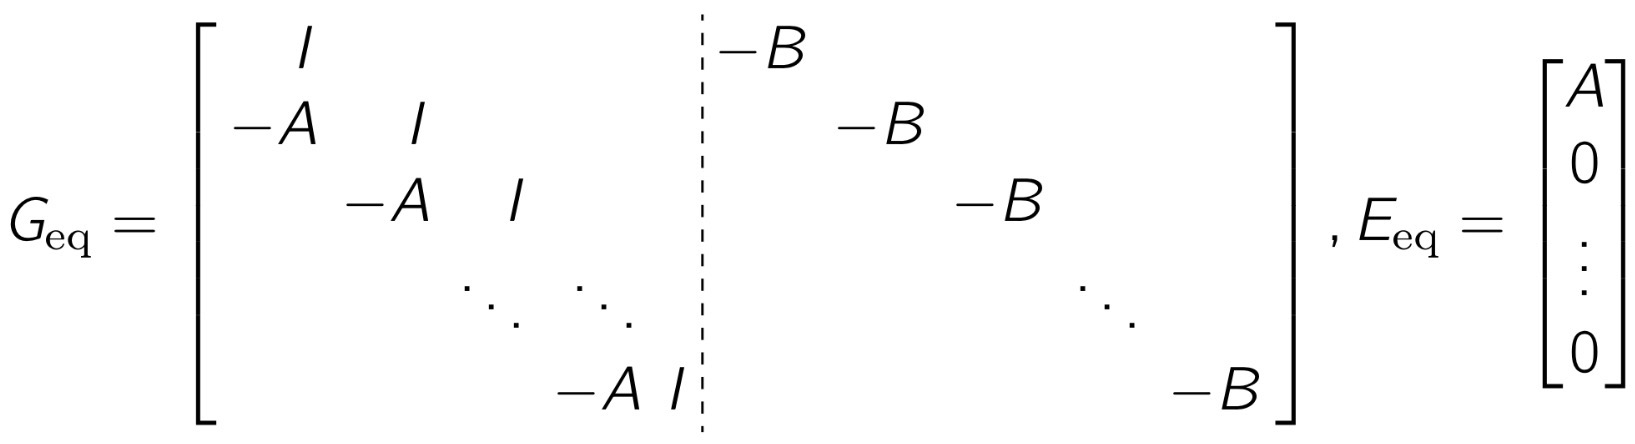
\includegraphics[width=0.49\linewidth]{images/CFTOC/without/equality.jpg} &
\includegraphics[width=0.39\linewidth]{images/CFTOC/without/inequality.jpg}\\
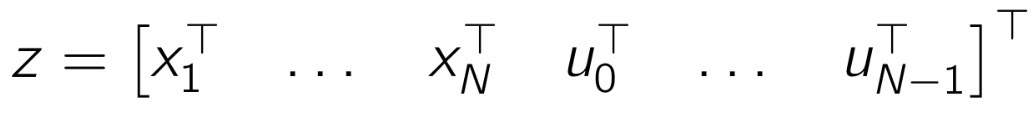
\includegraphics[width=0.29\linewidth]{images/CFTOC/without/z.jpg} &
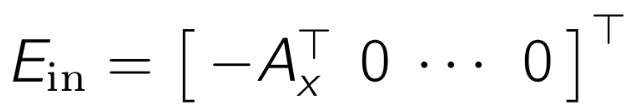
\includegraphics[width=0.19\linewidth]{images/CFTOC/without/E_in.jpg}
\end{tabular}
\end{center}
\vspace{-0.5em}
\subsubsection{With Substitution}
Idea: Substitute the state equations $x_{i+1}=Ax_i+Bu_i\;\;x_0=x(k)$
\begin{itemize}
    \item \textbf{Step 1}: Rewrite the cost as: \\
    $J(x(k),U)=U^THU+2\,x(k)^TFU+x(k)^TYx(k)$\\
    $J=\begin{bmatrix}U^T & x(k)^T\end{bmatrix} \begin{bmatrix}H & F^T \\F & Y\end{bmatrix}\begin{bmatrix}U^T& x(k)^T\end{bmatrix}^T$
    \item \textbf{Step 2}: Rewrite the constraints compactly: \\
    $GU\leq w\,+\,Ex(k)$\\
    Feasible sets: $\mathcal{X}=\{ x\,|A_xx\leq b_x\}$, $\mathcal{U}=\{ u\,|A_uu\leq b_u\}$, $\mathcal{X}_f=\{ x\,|A_fx\leq b_f\}$\\
    Reformulation:
    \begin{enumerate}
        \item $A_xx\leq b_x \rightarrow\;A_xS^UU\leq b_x-A_xS^xx(k)$
        \item $A_uU\leq b_u$
        \item $\boldsymbol{0}\leq b_x-A_xx(k)$\\
        $\rightarrow$ Build resulting $G,\, E\,$ and $w$.
    \end{enumerate}
\end{itemize}
\subsubsection{Comparisons}
$\forall\, \boldsymbol{x}\in \mathbb{R}^n,\,\boldsymbol{u}\in\mathbb{R}^m, horizon \rightarrow N$ 
{\small
\begin{tabularx}{\linewidth}{l|X|X}
 & WITH substitution & WITHOUT substitution \\
\hline
\# variables 
& $Nm$, $z=U$ 
& \makecell[l]{$N(m+n)$ \; $z=\begin{bmatrix}X & U\end{bmatrix}^T$} \\

Pros \& Cons 
& \makecell[l]{less variables \\ evtl. badly conditioned \\ extra computation}
& \makecell[l]{more variables \\ sparse} \\
\end{tabularx}
}


\subsubsection{$\infty$ and $1$ Norm Transformations (Reformulation in \textbf{epigraph} form)}
\noindent
\begin{minipage}[t]{0.48\linewidth}
\small
\begin{align*}
&\min_{x} \|x\|_\infty \text{ s.t. } Fx \leq g \\
&\Rightarrow \min_{x,t} t \text{ s.t. } Fx \leq g,\ -\mathbf{1}t \leq x \leq \mathbf{1}t
\end{align*}
\end{minipage}%
\hfill
\begin{minipage}[t]{0.48\linewidth}
\small
\begin{align*}
&\min_{x} \|x\|_1 \text{ s.t. } Fx \leq g \\
&\Rightarrow \min_{x,t} \mathbf{1}^T t \text{ s.t. } Fx \leq g,\ -t \leq x \leq t
\end{align*}
\end{minipage}


\subsection{Invariance}
\textbf{Constr. Control}:$\;x(k+1)=g(x(k),u(k))\;\forall x,u\in \mathcal{X},\mathcal{U}$\\
\textbf{Goal}: Find control law $u(k)=\kappa(x(k))$ s.t.
\begin{enumerate}
    \item $\{x(k)\}\subset\mathcal{X},\;\{u(k)\}\subset\mathcal{U}\;\;\forall k \rightarrow\textbf{Invariance}$
    \item Stability: $\lim_{k\rightarrow\infty}x(k)=0$
    \item Performance optimization
    \item Maximization of set: $\{x(0)|\;\;1-3\; satisfied\}$
\end{enumerate}
\textbf{Definitions}
\begin{enumerate}
    \item \textbf{Invariance}: Region s.t. the \textbf{autonomous system} (e.g. $x(k+1)=g(x(k))$) satisfies the constraints $\forall t$
    \item \textbf{Control Invariance}: Region in which there \textbf{exists a controller $\kappa$} (e.g. $x(k+1)=g(x(k),\kappa(x(k)))$) s.t. constraints are satisfied $\forall t$
\end{enumerate}


\textbf{Positively Invariant Set}\\ $\mathcal{O}$ is positively invariant for the \textbf{autonomous} system if $x(k)\in \mathcal{O} \Rightarrow x(k+1)\in \mathcal{O},\;\forall k\in\{0,1,...\}$\\
\textbf{Maximal Positively Invariant Set $\mathcal{O}_{\infty}$}\\
The set $\mathcal{O}_\infty\subset\mathcal{X}$ is a maximal positively invariant set w.r.t. $\mathcal{X}$ if:\\ 1) $\mathcal{O}_\infty$ is positively invariant and 2) it contains all positive invariant sets\\
\textbf{Pre Set} Given a set $S$ and the dynamics $x(k+1)=g(x(k))$, the pre set of S is: $pre(S):=\{x|\,g(x)\in S\}$\\
\textbf{e.g. Pre-set computation for linear autonomous systems}\\
Given set $S$ and dynamics $x(k+1)=Ax(k)$, then $pre(S):=\{x|\;Ax\in S\}$.\\
Assuming $S:=\{x|\;Fx\leq f\}\rightarrow pre(S)=\{x|\;FAx\leq f\}$\\
\textbf{Geometric condition for invariance}\\
Set $\mathcal{O}$ is positively invariant iff: $\mathcal{O}\subseteq pre(\mathcal{O}) \Leftrightarrow pre(\mathcal{O})\cap\mathcal{O}=\mathcal{O}$\\

\subsubsection{Algorithm to compute the maximal positively invariant set} $\mathcal{O}_\infty$ for $x(k+1)=g(x(k))$ \, \textbf{Input:} $g, \mathcal{X}$\, \textbf{Output:} $\mathcal{O}_\infty$\\
1. $\Omega_0 \leftarrow \mathcal{X}$\\
2. $\Omega_{i+1} \leftarrow \text{pre}(\Omega_i) \cap \Omega_i$\\
\hspace*{1em} \textbf{if} $\Omega_{i+1} = \Omega_i$ \textbf{then} \textbf{return} $\mathcal{O}_\infty = \Omega_i$ \textbf{else} repeat step 2.

\subsubsection{Control Invariance}
$\mathcal{C}\subseteq\mathcal{X}$ is control invariant if: $x(k)\in\mathcal{C}\Rightarrow\exists\;u(k)\in\mathcal{U}\; \text{s.t.}\;g(x(k),u(k))\in\mathcal{C}\;\;\forall k\in \mathbb{N}^+$\\
\textbf{Maximal Control Invariant Set $\mathcal{C_\infty}$}: $\mathcal{C}_\infty$ is maximal control invariant for $x(k+1)=g(x(k),u(k))$ if $\rightarrow$ 1) Control invariant and 2) contains all control invariant sets\\
\textbf{Calculation of Control invariant sets}:\\
Pre set $\rightarrow pre(S):=\{x|\;\exists u\in \mathcal{U}\ \text{s.t}\;g(x,u)\in S\}$\\

A set $\mathcal{C}$ is control invariant iff $\mathcal{C}\subseteq pre(\mathcal{C})$. Same algorithm as above
can be used.\\

\subsubsection{Pre Set Computation: Controlled system}
Given $x(k+1)=Ax(k)+Bu(k)$ with constraints $u(k)\in \mathcal{U}:=\{u|\;Gu\leq g\}$ and the set $S:=\{x| Fx\leq f\}$.\\
Then:
\begin{align*}
pre(S) &= \{x\,|\;\exists u\in\mathcal{U},\; Ax+Bu\in S\}\\
&= \{x\,|\;\exists u\in\mathcal{U},\; FAx+FBu\leq f\}\\
&= \left\{ x \;\middle|\; \exists u,\;
\begin{bmatrix}FA & FB \\ 0 & G\end{bmatrix}
\begin{bmatrix}x \\ u \end{bmatrix}
\leq
\begin{bmatrix}f \\ g\end{bmatrix}
\right\}
\end{align*}
$\rightarrow$ \textbf{projection operation}\\
\textbf{From Control invariant set $\rightarrow$ Control law}:
Synthesizing a control law $\kappa(x)$ from a control invariant set through optimization problem below:\\
$\kappa(x):=\text{argmin}_u\{f(x,u)|\;g(x,u)\in\mathcal{C},u\in\mathcal{U}\}$\\
NB: 1)$f(x,u)$ is any function, 2) system satisfies constraints but doesn't necessarily converge.\\
Control invariant set is a \textbf{powerful object}, and \textbf{if computable} it provides a direct method for determining a control law satisfying the constraints.\\
\textbf{Issue}: They are \textbf{not always computable} $\rightarrow$ MPC implicitly describes a control invariant set well representable and computable.

\subsection{Practical Computation of invariant sets}

\subsubsection{Polytopes}
  \textbf{Convex hull}: for any subset $S\in\mathbb{R}^d$, co($S$) of S $\rightarrow$ intersection of all convex sets containing S (\textit{smallest convex set containing $S$})\\
  \textbf{Proposition: Convex hull}: convex hull of a set of points $\{v_1,...,v_k\}\in\mathbb{R}^d\rightarrow \text{co($\{v_1,...,v_k\}$}):=\{x|\;x=\sum_i\lambda_iv_i\;,\;\lambda_i\geq0\;,\;\sum_i\lambda_i=1\;\forall i=1,...,k\}$\\
  \textbf{Minkowski-Weyl Theorem}: For $P\subseteq\mathbb{R}^d$ the statements below are equivalent:\\
  \begin{enumerate}
      \item $P$ is a polytope (i.e. $\exists\; A\in\mathbb{R}^{m\,\text{x}\,d},\;b\in\mathbb{R}^m \;\text{s.t.}\;P=\{x|\;Ax\leq b\}$)
      \item $P$ is finitely generated (i.e. $\exists\;\{v_i\}\;\text{s.t.}\; P=\text{co}(\{v_1,...,v_s\})$)
  \end{enumerate}
  \textbf{Examples: Polytopes in MPC}\\
  \begin{itemize}
  \item\textbf{Rate constraints}:\\$||x(k)-x(k+1)||_\infty\leq \alpha\;\Rightarrow\;\begin{bmatrix}I & -I \\ -I & I\end{bmatrix}\begin{bmatrix}x(k) \\ x(k+1)\end{bmatrix}\leq \boldsymbol{1}\alpha$\\
  $\rightarrow$ Polytopes in MPC commonly desribed by \textbf{inequalities}
  \end{itemize}
\textbf{Intersection of Polytopes}: \\Intersection $I\subseteq\mathbb{R}^n$ of sets $S\subseteq\mathbb{R}^n, \;T\subseteq\mathbb{R}^n\;\rightarrow\;I=S\cap T:=\{x|\;x\in S \;\text{and}\; x\in T\}$\\
\textbf{Subset Test}: Is $P:=\{x|\;Cx\leq c\}$ contained in $Q:=\{x|\;Dx\leq d\}$ ?\\ $\rightarrow$ \textbf{True} if $P\subset\{x|\;D_ix\leq d_i\}$ for each row $D_i$ of $D$\\
$\rightarrow$ \textbf{support function} of the set P: $h_P(D_i):=\text{max}_x\,D_ix\;\;\text{subj. to}\;Cx\leq c$ ($h_P(D_i)\leq d_i\;\forall i$)\\

\subsubsection{Ellipsoids}
\textbf{Ellipse}: $E:=\{x|\;(x-x_c)^TP(x-x_c)\leq1\}$ with P$\succeq0$ sym. in $\mathbb{R}^{n\,\text{x}\,n}$ and $x_c\in \mathbb{R}^n$
\textbf{Lemma: Invariant set from Lyapunov function}: $V:\mathbb{R}^n\rightarrow\mathbb{R}$ is a Lyapunov fct. for the system $x(k+1)=g(x(k))$, then $Y:=\{x|\;V(x)\leq \alpha\}$ is \textbf{invariant} $\forall\;\alpha\geq0$\\
\textbf{Goal}: find largest $\alpha$ s.t.:$Y_\alpha:=\{x|\;x^TPx\leq \alpha\}\subset\mathcal{X}:=\{x|\;Fx\leq f\}$\\

\textbf{Maximum ellipsoidal invariant set}: largest ellipsoid contained in a polytope, with
\[
\alpha^\star=\max_\alpha\{\alpha\mid \|P^{-1/2}F_i^\top\|^2\alpha\le f_i^2,\ \forall i\}=\min_i\frac{f_i^2}{F_iP^{-1}F_i^\top}.
\]


\subsection{Feasibility and Stability}
\textbf{Potential issues} with MPC:
\begin{enumerate}
    \item \textbf{No feasibility guarantee} \rightarrow MPC evtl. has no solution
    \item \textbf{No stability guarantee} \rightarrow Trajectories evtl. do not converge to origin
\end{enumerate}

\begin{center}
\scriptsize
\setlength{\tabcolsep}{5pt}
\renewcommand{\arraystretch}{1.15}
\begin{tabular}{|
>{\centering\arraybackslash}m{0.14\linewidth}|
>{\centering\arraybackslash}m{0.35\linewidth}|
>{\centering\arraybackslash}m{0.41\linewidth}|}
\hline
\textbf{Horizon} & \textbf{Feasibility} & \textbf{Stability / Cost} \\ \hline
$N\to\infty$
& Closed-loop trajectory always feasible
& As in LQR: open loop = closed loop; finite cost
  $\Rightarrow x_k,u_k\to0$ \\ \hline
Finite $N$
& Finite-horizon OCP may become infeasible
& Inputs may not drive the system to the origin \\ \hline
\end{tabular}
\end{center}

Issues caused by use of \rightarrow \textbf{short sighted strategies}\\
\textbf{Goal}: Design finite horizon \rightarrow approximate infinite horizon\\
\textbf{Idea}: Introduce terminal cost and constraints to ensure feasibility and stability (\textcolor{red}{mimic infinite horizon})
$J^*(x(k))= \text{min}_U \;\textcolor{red}{l_f(x_N)}\;+\;\sum_{i=0}^{\textcolor{red}{N}-1}l(x_i,u_i)$, $\textcolor{red}{x_N}\in\textcolor{red}{\mathcal{X}_f}$\\

\textbf{Recursive feasibility}: showing the existence of a feasible control sequence at all times when starting from a feasible initial point\\
\textbf{Stability}: showing that the optimal cost function is a Lyapunov function, were \textbf{proven in lecture}:\\ 
for cases: 1) Terminal constraint: $x_N=0$, 2) Terminal constraint in some convex set $x_N\in\mathcal{X}_N$\\


\subsubsection{Lyapunov Stability}
\begin{itemize}
    \item Asymptotic stability: Eqb. point $\bar{x}\in\Omega$ is asy. stable in the set $\Omega\in\mathbb{R}^n$ if it is Lyap. stable and \textbf{attractive}, i.e.
    $\text{lim}_{k\rightarrow\infty}\;||x(k)-\bar{x}||=0\,,\;\forall x(0)\in\Omega$\\
    \textbf{Global asy. stability} if asy. stable and $\Omega=\mathbb{R}^n$
    \item Lyapunov fct.: Fct. $V:\mathbb{R}^n\rightarrow\mathbb{R}$ s.t.$V(0)=0\; \text{and}\;V(x)>0\; \forall x\in\Omega\backslash\{0\}$\\
    $V(g(x))-V(x)\leq-\alpha(x)\;\forall x\in\Omega\backslash\{0\}$, $\alpha(x):\mathbb{R}^n\rightarrow\mathbb{R}$
    \item Lyapunov (asy.) stability: For systems admitting Lyap. fcts. $V(x)$, $x=0$ is \textbf{asymptotically stable} in $\Omega$
\end{itemize}
\subsubsection{Feasibility and stability guarantees proof for $\mathcal{X}_\text{f}=0$}
\begin{enumerate}
\item Goal: Prove recursive feasibility
\begin{itemize}
    \item Assume feasibility of $x(k)$ and $\{u_0^*\,,\,u_1^*\,,\,...\,,\,u_{N-1}^*\}$ optimal control sequence at $x(k)$ with $\{x(k)\,,\,x_1^*\,,\,...\,,\,x_{N}^*\}$ corresponding state trajectory
    \item Apply $u(k)=u_0^*$ and let the system evolve to $x(k+1)=A\,x(k)+B\,u(k)=x_1^*$
    \item At $x(k+1)$ the control sequence $\tilde{U}=\{u_1^*\,,\,u_2^*\,,...\,,u_{N-1}^*\,,\textcolor{red}{0}\}$ is \textbf{feasible}.\\
    $A\,x_N^*+B\cdot0=0$ \Rightarrow Feasible set is invariant, terminal constraint is satisfied, Feasible set is invariant \rightarrow \textcolor{red}{Recursive feasibility}
\end{itemize}
\item Goal: Show $J^*(x(k+1))<J^*(x(k))\;\forall x(k)\neq0$\\
$\tilde{U}=\{u_1^*\,,\,u_2^*\,,...\,,u_{N-1}^*\,,\textcolor{red}{0}\}$, $\tilde{X}=\{x_1^*\,,\,...\,,\,x_{N}^*\,,\,\textcolor{red}{0}\}$\\
$J^*(x(k))=l_f(x_N^*)+\sum_{i=0}^{N-1}l(x_i^*\,,\,u_i^*)\,,\text{with }l_f(x_N^*)=0$\\
$J^*(x(k+1))\leq\tilde{J}(x(k+1))=\sum_{i=1}^{N-1}l(x_i^*\,,\,u_i^*)+l(x_N^*\,,\,0)$\\
$=\sum_{i=0}^{N-1}l(x_i^*\,,\,u_i^*)-l(x_0^*\,,\,u_0^*)+l(x_N^*\,,\,0)$\\
$=J^*(x(k))-l(x(k)\,,\,u_0^*)+l(0\,,\,0)\;\text{where }l(0\,,\,0)=0$\\
\Rightarrow $J^*(x)$ is a \textcolor{red}{Lyapunov function} \rightarrow \textcolor{red}{Asymptotic Lyapunov stability}
\end{enumerate}
\textbf{Extension to more general terminal sets}\\
\textbf{Problem:} The constraint $x_N=0$ reduces the size of the feasible set\\
\textbf{Goal:} Make use of $\mathcal{X}_f$ to increase the region of attraction \\\rightarrow Generalize proof to the constraint $x_N\in\mathcal{X}_\text{f}$\\

\textbf{Def: Invariant set}\\
$\mathcal{O}\rightarrow \textbf{positively invariant}$ for $x(k+1)=g_{cl}(x(k))$ if:\\
$x(0)\in\mathcal{O}\Rightarrow x(k)\in\mathcal{O}, \;\forall k\in\mathbb{N}_+$\\
\subsubsection{Stability of MPC - Main results}
Assumptions (\textbf{sufficient} conditions that guarantee stability and feasibility of the MPC)
\begin{enumerate}
    \item \textbf{Positive definite stage cost} (strictly pos. and only zero at the origin)
    \item \textbf{Recursive Feasibility}: Terminal set is \textbf{invariant} under the local control law $\kappa_\text{f}(x_i)$:\\
    $x_{i+1}=A\,x_i+B\kappa_\text{f}(x_i)\in\mathcal{X}_\text{f},\;\forall x_i\in\mathcal{X}_\text{f}$\\
    All state and input constraints are satisfied:\\
    $\mathcal{X}_\text{f}\subseteq\mathcal{X}\,,\,\kappa_\text{f}(x_i)\subseteq\mathcal{U},\;\forall x_i\in\mathcal{X}_\text{f}$
    \item \textbf{Stability}: Terminal cost is a continuous \textbf{Lyapunov function} in the terminal set $\mathcal{X}_\text{f}$ and:\\
    $l_\text{f}(x_{i+1})-l_\text{f}(x_i)\leq-l(x_i\,,\,\kappa_\text{f}(x_i))$
\end{enumerate}
Plan for N steps \rightarrow use local controller that keeps the system in a stable manner in the terminal set (condition 3 ensures stability)\\
\textbf{Theorem (Closed-Loop System Stability)}:\\
Under those 3 assumptions, the closed-loop system under the MPC control law $u_0^*(x)$ is asymptotically stable and the set $\mathcal{X}_\text{N}$ (Region of Attraction) is positively invariant for the system\\
$x(k+1)=A\,x(k)+B\,u_0^*(k)$\\
\textbf{Stability of MPC - Outline of the Proof}\\
\begin{itemize}
    \item Assume feasibility of $x(k)$ and $\{u_0^*\,,\,...\,,\,u_{N-1}^*\}$ the optimal control sequence computed at $x(k)$ with $\{x(k)\,,\,x_1^*\,,\,...\,,\,x_N^*\}$ the resulting state trajectory
    \item At $x(k+1)=x_1^*$ the sequence: $\tilde{U}=\{u_1^*\,,\,...\,,\,\kappa_\text{f}(x_N^*)\}$ is \textbf{feasible} ($x_N^*\in\mathcal{X}_\text{f}$\rightarrow $\kappa_\text{f}(x_N^*)$ is feasible and $A\,x_N^*+B\,\kappa_\text{f}(x_N^*)\in\mathcal{X}_\text{f}$)\\
    \Rightarrow Terminal constraint provides \textcolor{red}{Recursive feasibility}
\end{itemize}
\textbf{Asymptotic stability of MPC - Outline of the proof}\\
$J^*(x(k))=\sum_{i=0}^{N-1}l(x_i^*\,,\,u_i^*)+l_\text{f}(x_N^*)$\\
At $x(k+1)=x_1^*\,,\,\tilde{U}=\{u_1^*\,,\,...\,,\,\kappa_\text{f}(x_N^*)\}$ is feasible and sub-optimal:\\
$J^*(x(k+1))\leq\sum_{i=1}^{N-1}l(x_i^*\,,\,u_i^*)+l(x_N^*\,,\,\kappa_\text{f}(x_N^*))+l_\text{f}(A\,x_N^*+B\,\kappa_\text{f}(x_N^*))$\\
$=\sum_{i=0}^{N-1}l(x_i^*\,,\,u_i^*)-l(x_0^*\,,\,u_0^*)+l(x_N^*\,,\,\kappa_\text{f}(x_N^*))+l_\text{f}(A\,x_N^*+B\,\kappa_\text{f}(x_N^*))$\\
$=J^*(x(k))-l(x(k)\,,\,u_0^*)+l_\text{f}(A\,x_N^*+B\,\kappa_\text{f}(x_N^*))-l_\text{f}(x_N^*)+l(x_N^*\,,\,\kappa_\text{f}(x_N^*))$\\
$\Rightarrow J^*(x(k+1))-J^*(x(k))\leq-l(x(k)\,,\,u_0^*)$\\
\textcolor{red}{$J^*(x)$ \textbf{ is a Lyapunov function}}\\
\Rightarrow The closed-loop system under the MPC control law is \textcolor{red}{asymptotically stable}\\
\subsubsection{Choice of terminal sets and cost - Linear system dynamics and quadratic cost}
$J^*(x(k))=\min_U\textcolor{red}{x_N^TPx_N}+\sum_{i=0}^{\textcolor{red}{N}-1}x_i^TQx_i+u_i^TRu_i$ (\textcolor{red}{Terminal cost})\\
subj.to  $x_{i+1}=A\,x_i+B\,u_i, \forall i=0\,,\,...\,,\,N-1$\\
$x_i\in\mathcal{X}\,,\,u_i\in\mathcal{U}\,,\,\forall i=0\,,\,...\,,\,N-1$\\
$\textcolor{red}{x_N\in\mathcal{X}_\text{f}}$ (\textcolor{red}{Terminal constraint})\\
$x_0=x(k)$\\
\begin{itemize}
    \item Formulate unconstrained LQR control law:\\
    $F_\infty=-(B^TP_\infty B+R)^{-1}B^TP_\infty A$\\
    $P_\infty \rightarrow $ solution to DARE
    \item Terminal weight $P=P_\infty$
    \item Terminal set $\mathcal{X}_\text{f}$ maximum invariant set for the cl-system $x_{k+1}=(A+BF_\infty)x_k$\\
    $x_{k+1}=(A+BF_\infty)x_k\in\mathcal{X}_\text{f},\;\forall x_k\in \mathcal{X}_\text{f}$\\
    $\mathcal{X}_\text{f}\subseteq\mathcal{X}\,,\, F_\infty x_k\subseteq\mathcal{U}\,\,\forall x_k\in\mathcal{X}_\text{f}$
\end{itemize}
\begin{enumerate}
    \item Stage cost is positive definite
    \item Terminal set is invariant by construction under the local control law $\kappa_\text{f}(x)=F_\infty x$
    \item Terminal cost is continuous Lyapunov function in the terminal set $\mathcal{X}_\text{f}$ and:\\
    $x_{k+1}^TP_\infty x_{k+1}-x_k^TP_\infty x_k=$\\
    $x_k^T(-P_\infty+A^TP_\infty A+F_\infty^TB^TP_\infty A-F_\infty^TRF_\infty)x_k$\\
    $=-x_k^T(Q+F_\infty^TRF_\infty)x_k$
\end{enumerate}
\rightarrow All assumptions of the feasibility and stability theorem are verified\\


\begingroup

\textbf{Example}:
\begin{enumerate}
    \item Compute the optimal LQR controller and cost matrices:
    $F_\infty,\;P_\infty$.
    
    \item Compute the maximal invariant set $\mathcal{X}_{\mathrm f}$
    for the closed-loop system
    $x_{k+1}=(A+BF_\infty)x_k$, subject to
    \[
    \mathcal{X}_{\mathrm{cl}}
    :=
    \left\{
    x \,\middle|\,
    \begin{bmatrix}
        A_x\\
        A_uF_\infty
    \end{bmatrix}x
    \le
    \begin{bmatrix}
        b_x\\
        b_u
    \end{bmatrix}
    \right\}.
    \]
\end{enumerate}

\endgroup
\textbf{Summary}
\begin{itemize}
    \item Terminal constraint \textbf{sufficient} condition for feasibility and stability
    \item Region of attraction (ROA) without terminal constraint evtl. larger than for MPC with terminal constraint
    \item $\mathcal{X}_\text{f}=0$ simplest choice \rightarrow small ROA for small N
    \item Solutions available for linear systems with quadratic cost
    \item Practically: Enlarge horizon $N$, check stability by sampling
    \item Larger horizon $N$\rightarrow ROA reaches maximum control invariant set
\end{itemize}
\textbf{Sidenotes}: 
\begin{itemize}
    \item From example: Decrease in the prediction horizon causes loss of the stability properties
    \item Inclusion of the terminal cost and constraint provides stability
\end{itemize}
\textbf{Extension to nonlinear MPC}\\
Given nonlinear system dynamics $x(k+1)=g(x(k)\,,\,u(k))$\\
\rightarrow Assumptions on terminal set and constraints: NOT relying on linearity
\rightarrow Lyapunov stability used to analyze stability of nonlinear dynamical systems\\
Issue: determining $\mathcal{X}_\text{f}$ and $l_\text{f}$ can be difficult\\
\textbf{Summary}\\
\textbf{Finite-horizon MPC may not be stable}\\
\textbf{Finite-horizon MPC may not satisfy the constraints for all time}\\
\textcolor{red}{\rightarrow} in contrast infinite-horizon provides stability and invariance\\
\textcolor{red}{\rightarrow} Infinite-horizon faked by: forcing final state to be in invariant set for which there is an invariance-inducing controller


\endgroup